
%%%%%%%%% MASTER -- compiles the 4 sections

%\documentclass[12pt,letterpaper]{article}
\documentclass[12pt,letterpaper,headings=normal]{scrartcl}

%%%%%%%%%%%%%%%%%%%%%%%%%%%%%%%%%%%%%%%%%%%%%%%%%%%%%%%%%%%%%%%%%%%%%%%%%
\pagestyle{plain}                                                      %%
%%%%%%%%%% EXACT 1in MARGINS %%%%%%%                                   %%
\setlength{\textwidth}{6.5in}     %%                                   %%
\setlength{\oddsidemargin}{0in}   %% (It is recommended that you       %%
\setlength{\evensidemargin}{0in}  %%  not change these parameters,     %%
\setlength{\textheight}{8.5in}    %%  at the risk of having your       %%
\setlength{\topmargin}{-.3in}       %%  proposal dismissed on the basis  %%
\setlength{\headheight}{0in}      %%  of incorrect formatting!!!)      %%
\setlength{\headsep}{0in}         %%                                   %%
\setlength{\footskip}{.2in}       %%                                   %%
%%%%%%%%%%%%%%%%%%%%%%%%%%%%%%%%%%%%                                   %%
\newcommand{\required}[1]{\section*{\hfil #1\hfil}}                    %%
\renewcommand{\refname}{\hfil References Cited\hfil}                   %%
\bibliographystyle{plain}                                              %%
%%%%%%%%%%%%%%%%%%%%%%%%%%%%%%%%%%%%%%%%%%%%%%%%%%%%%%%%%%%%%%%%%%%%%%%%%

%\setlength{\textheight}{9.4in}
%\renewcommand{\topfraction}{1}		% max fraction of floats at top
%\renewcommand{\bottomfraction}{1}	% max fraction of floats at bottom
%\def\overheader{-0.1in}
%\def\underheader{-0.1in}

\renewcommand{\rmdefault}{ptm} % Palatino=ppl or Times=ptm
\renewcommand{\sfdefault}{phv} % Helvetica
\renewcommand{\ttdefault}{pcr}  % Courier

\renewcommand{\thesection}{\Alph{section}} % change section nunbering to alphabetic

%PUT YOUR MACROS HERE
\usepackage{comment}
\usepackage{subfigure}
\usepackage{graphicx}
\usepackage{wrapfig}
\usepackage{url}
\usepackage{multicol}
\usepackage[margin=0pt,font=small,labelfont=bf,format=plain]{caption}
\usepackage{fancyhdr}
\usepackage{datetime}
\pagestyle{fancy}
\fancyhf{}
\renewcommand{\headrulewidth}{0pt}
\fancyhead[R]{\vspace{-1.5cm} \textit{Page =}~\thepage}
\usepackage{pdfpages}
\includepdfset{pagecommand=\thispagestyle{fancy}}
\usepackage{epsfig}


\begin{document}

%\markboth{\Large \bf Revised handout}{ }

%\baselineskip=24pt  % Enforce double space

\baselineskip=48pt  % Enforce double space

%\baselineskip=18pt  % Enforce 1.5 space
%
%\setlength{\parskip}{.3in}
%\setlength{\itemsep}{.3in}

\pagestyle{plain}

\vspace*{7cm}


\begin{center}
{\Large
ROB 501 Handouts \\
RLS, BLUE and MVE
\mbox{ } \\
J.W. Grizzle \\
\mbox{ } \\
}
%{\bf Compiled on~\today~~at~\currenttime}
\end{center}



\newpage
\vspace*{10cm}
{\Large
\begin{center}
Recursive Least Squares, Best Linear Unbiased Estimator, and Minimum Variance Estimators \\
\mbox{ } \\
\end{center}
}
\newpage

\textbf{Sources:}
{\footnotesize
\begin{itemize}
\item Recursive Least Squares\\
\url{http://ocw.mit.edu/courses/electrical-engineering-and-computer-science/6-241j-dynamic-systems-and-control-spring-2011/readings/MIT6_241JS11_chap02.pdf}
\item Simplified Presentation of Various Estimators \\
\url{http://home.engineering.iastate.edu/~namrata/EE527_Spring08/l3.pdf} \\
(See also) \url{http://home.engineering.iastate.edu/~namrata/EE527_Spring12/}
\item  Higher Level Summary of Various Estimators. Heavily Based on the Projection Theorem\\
\url{http://www4.ncsu.edu/~mtchu/Teaching/Lectures/MA719/chapter4.pdf}
\end{itemize}
}
\newpage

\vspace*{\fill}
Recursive Least Squares (See Section 2.6). \\
Notational changes we make in lecture with respect to the handout:\\
$$\bar{S} \to R$$
$$\bar{y} \to Y$$
$$\bar{A} \to A$$
$$A_i \to C_i$$
\vspace*{\fill}
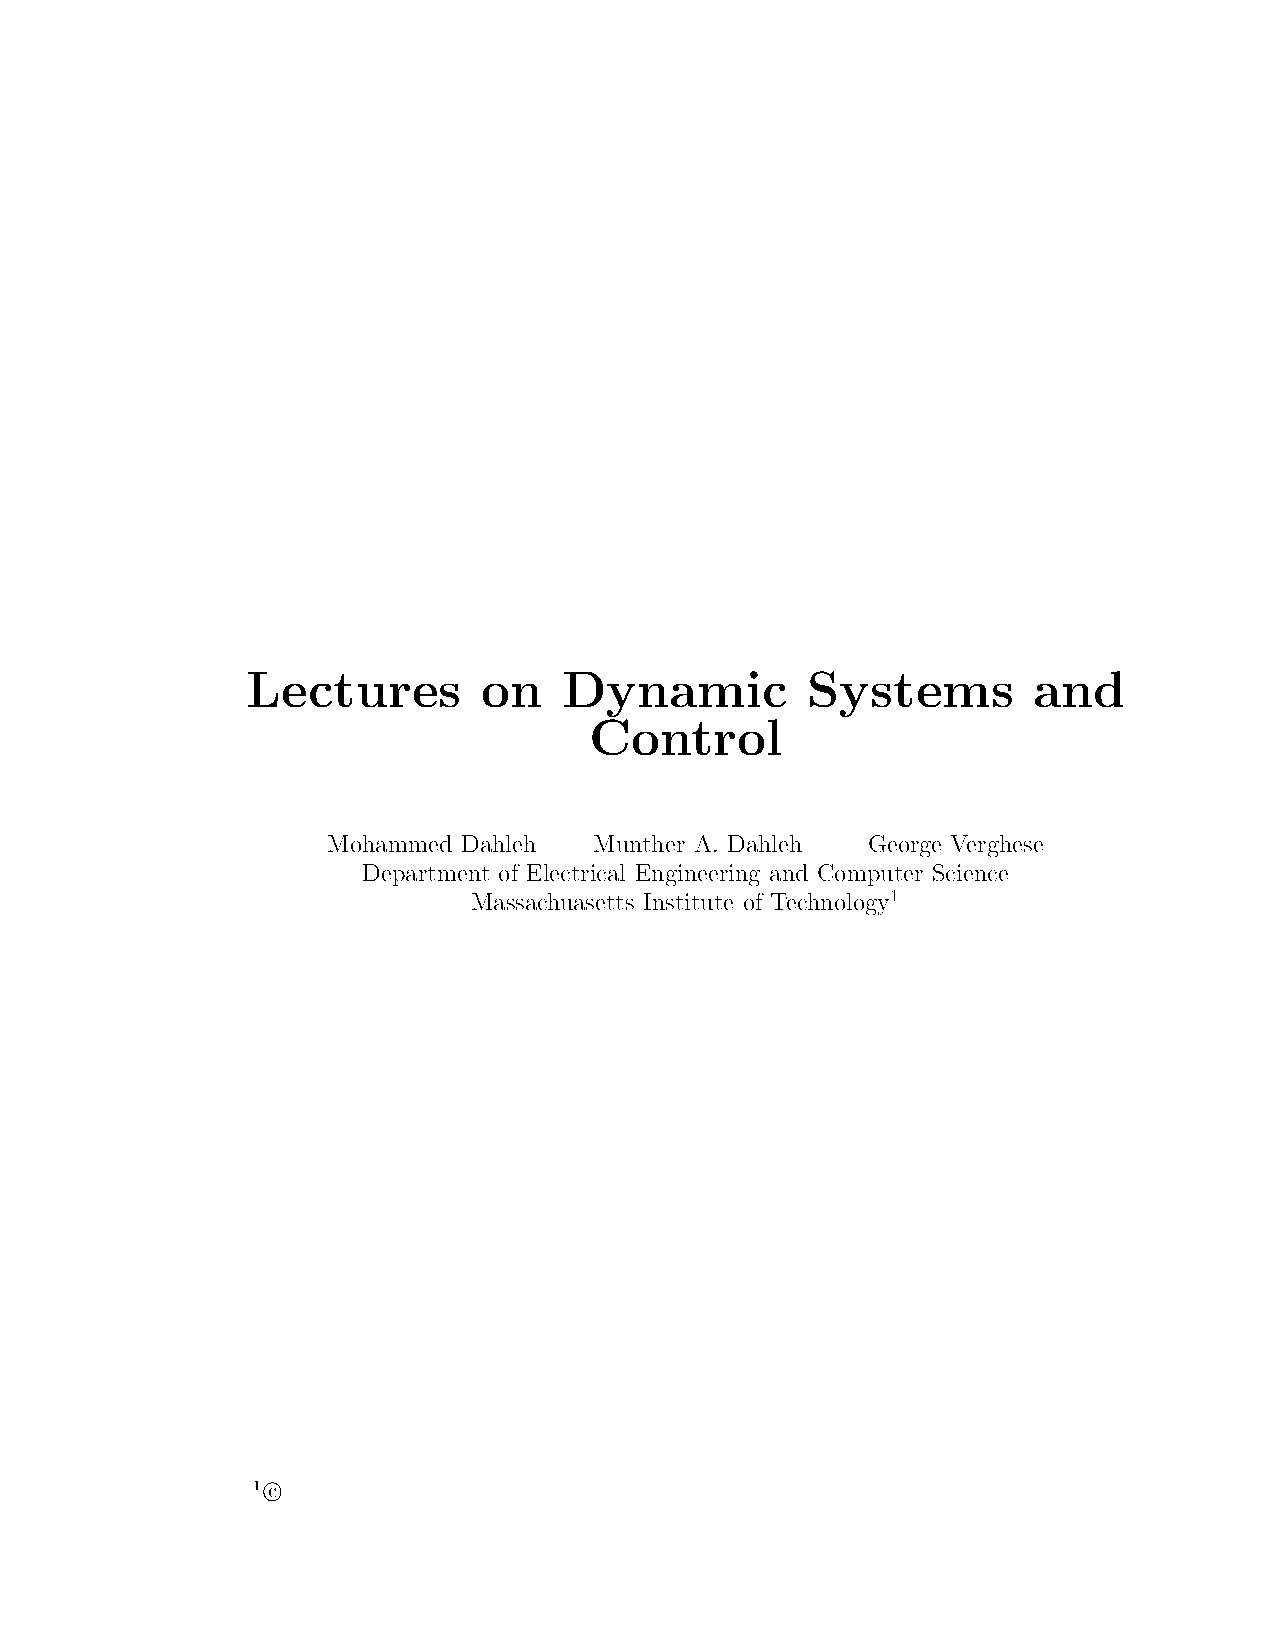
\includepdf[pages=-]{NotesFromWeb/LeastSquares/LeastSquaresEstimation_MIT6_241JS11_chap02.pdf}
\vspace*{\fill}
Simplified Presentation of BLUE (Best Linear Unbiased Estimators) \\and \\MVE (Minimum Variance Estimators)\\
(Ignore material on Maximum Likelihood)
\vspace*{\fill}
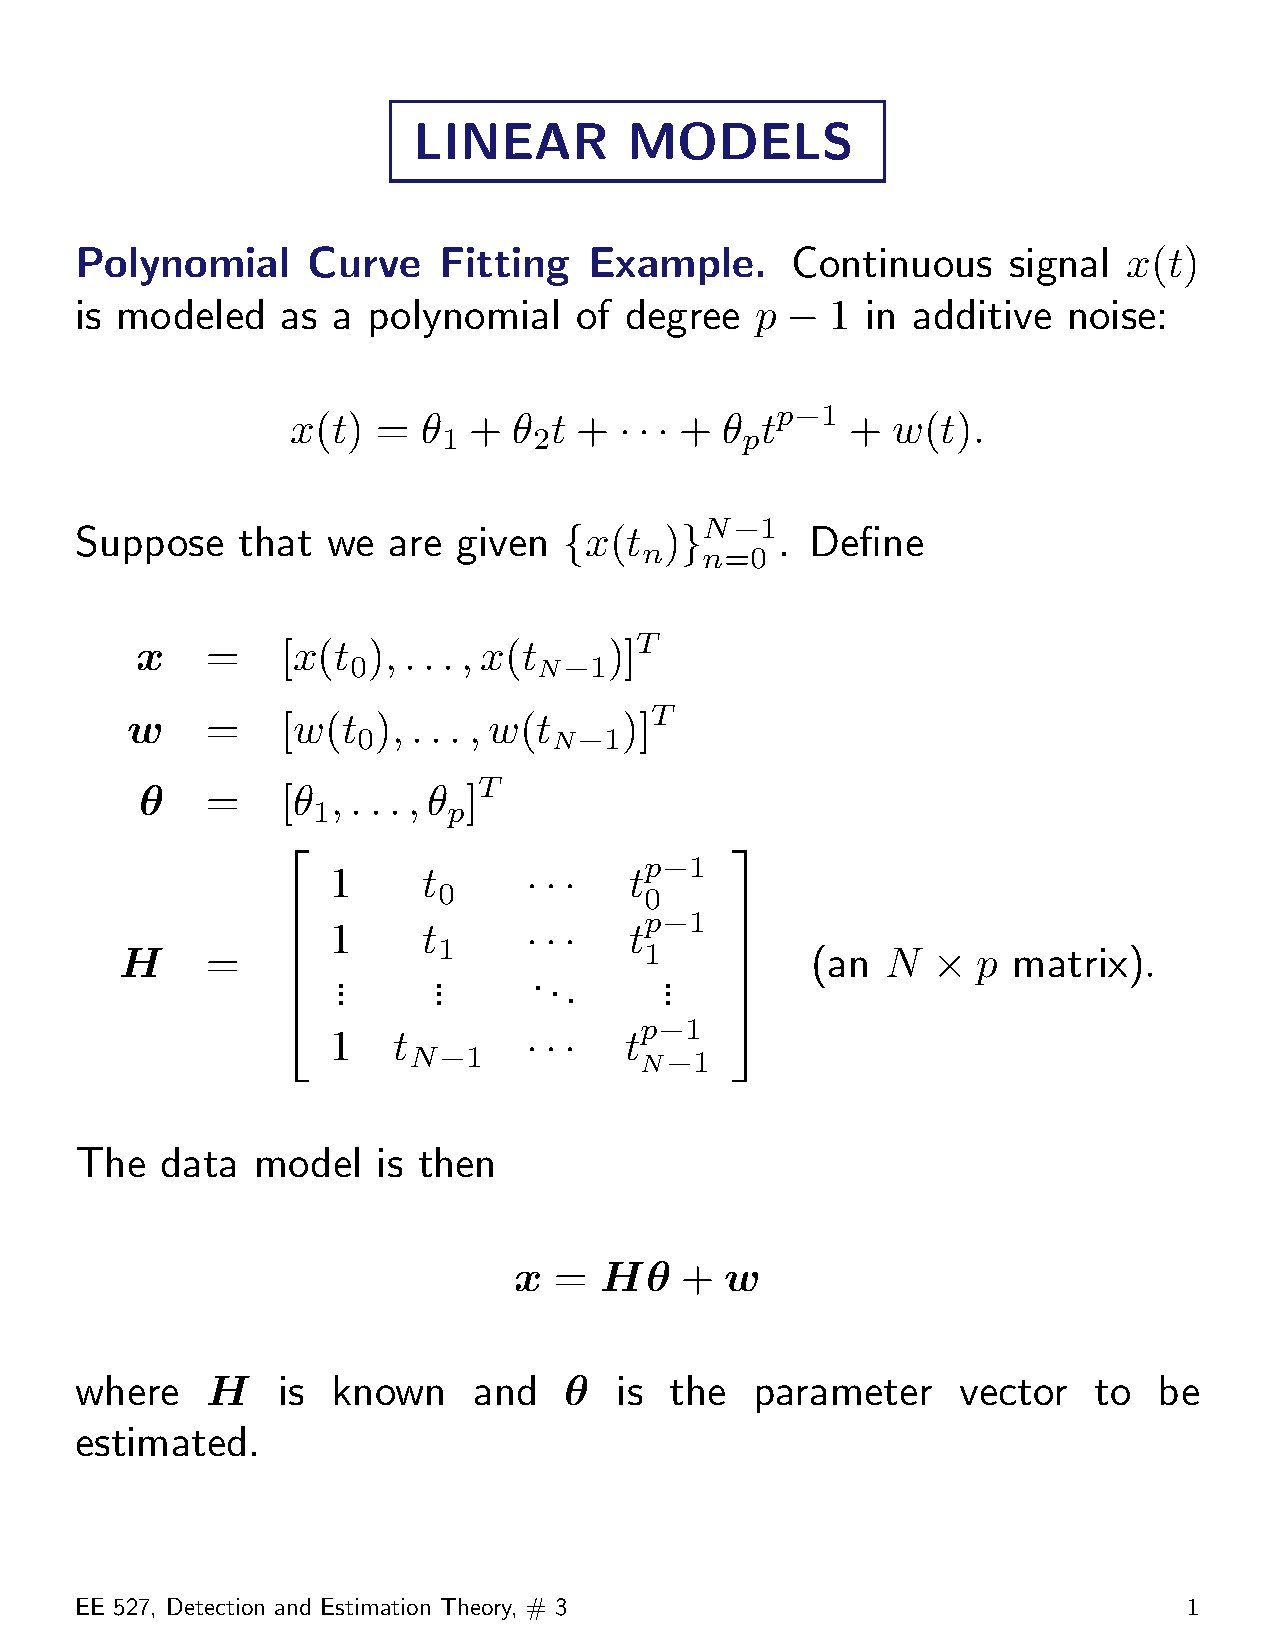
\includepdf[pages=1-15]{NotesFromWeb/EstimationAndKalmanFilter/BLUE.pdf}
\vspace*{\fill}
Based on Chapter 4 of Luenberger, ``Optimization by Vector Space Methods''. Based on the Projection Theorem. Has a short probability review as well.
\vspace*{\fill}
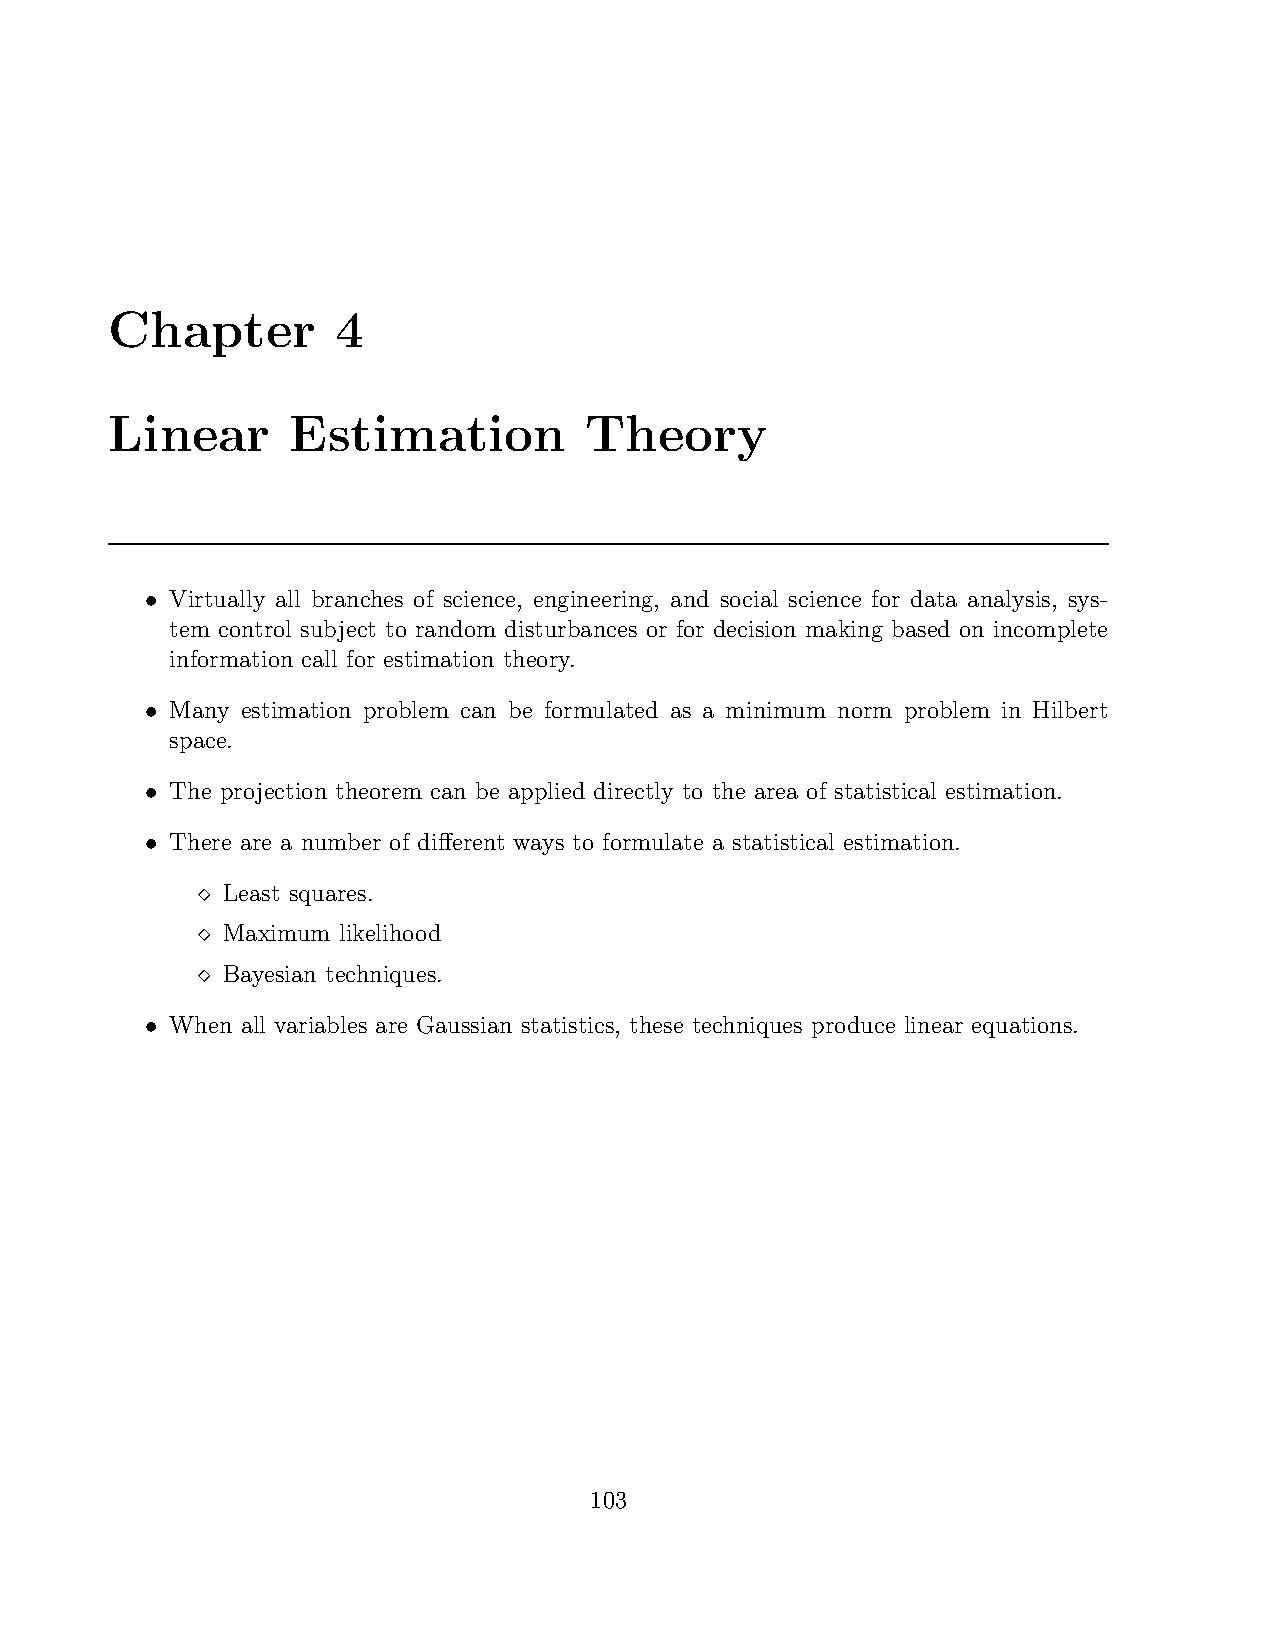
\includepdf[pages=-]{NotesFromWeb/LeastSquares/LeastSquaresEstimation_chapter4[LuenbergerStuff].pdf}


\end{document}
